% Options for packages loaded elsewhere
\PassOptionsToPackage{unicode}{hyperref}
\PassOptionsToPackage{hyphens}{url}
\PassOptionsToPackage{dvipsnames,svgnames,x11names}{xcolor}
%
\documentclass[
  letterpaper,
  DIV=11,
  numbers=noendperiod]{scrartcl}

\usepackage{amsmath,amssymb}
\usepackage{iftex}
\ifPDFTeX
  \usepackage[T1]{fontenc}
  \usepackage[utf8]{inputenc}
  \usepackage{textcomp} % provide euro and other symbols
\else % if luatex or xetex
  \usepackage{unicode-math}
  \defaultfontfeatures{Scale=MatchLowercase}
  \defaultfontfeatures[\rmfamily]{Ligatures=TeX,Scale=1}
\fi
\usepackage{lmodern}
\ifPDFTeX\else  
    % xetex/luatex font selection
\fi
% Use upquote if available, for straight quotes in verbatim environments
\IfFileExists{upquote.sty}{\usepackage{upquote}}{}
\IfFileExists{microtype.sty}{% use microtype if available
  \usepackage[]{microtype}
  \UseMicrotypeSet[protrusion]{basicmath} % disable protrusion for tt fonts
}{}
\makeatletter
\@ifundefined{KOMAClassName}{% if non-KOMA class
  \IfFileExists{parskip.sty}{%
    \usepackage{parskip}
  }{% else
    \setlength{\parindent}{0pt}
    \setlength{\parskip}{6pt plus 2pt minus 1pt}}
}{% if KOMA class
  \KOMAoptions{parskip=half}}
\makeatother
\usepackage{xcolor}
\setlength{\emergencystretch}{3em} % prevent overfull lines
\setcounter{secnumdepth}{-\maxdimen} % remove section numbering
% Make \paragraph and \subparagraph free-standing
\makeatletter
\ifx\paragraph\undefined\else
  \let\oldparagraph\paragraph
  \renewcommand{\paragraph}{
    \@ifstar
      \xxxParagraphStar
      \xxxParagraphNoStar
  }
  \newcommand{\xxxParagraphStar}[1]{\oldparagraph*{#1}\mbox{}}
  \newcommand{\xxxParagraphNoStar}[1]{\oldparagraph{#1}\mbox{}}
\fi
\ifx\subparagraph\undefined\else
  \let\oldsubparagraph\subparagraph
  \renewcommand{\subparagraph}{
    \@ifstar
      \xxxSubParagraphStar
      \xxxSubParagraphNoStar
  }
  \newcommand{\xxxSubParagraphStar}[1]{\oldsubparagraph*{#1}\mbox{}}
  \newcommand{\xxxSubParagraphNoStar}[1]{\oldsubparagraph{#1}\mbox{}}
\fi
\makeatother


\providecommand{\tightlist}{%
  \setlength{\itemsep}{0pt}\setlength{\parskip}{0pt}}\usepackage{longtable,booktabs,array}
\usepackage{calc} % for calculating minipage widths
% Correct order of tables after \paragraph or \subparagraph
\usepackage{etoolbox}
\makeatletter
\patchcmd\longtable{\par}{\if@noskipsec\mbox{}\fi\par}{}{}
\makeatother
% Allow footnotes in longtable head/foot
\IfFileExists{footnotehyper.sty}{\usepackage{footnotehyper}}{\usepackage{footnote}}
\makesavenoteenv{longtable}
\usepackage{graphicx}
\makeatletter
\def\maxwidth{\ifdim\Gin@nat@width>\linewidth\linewidth\else\Gin@nat@width\fi}
\def\maxheight{\ifdim\Gin@nat@height>\textheight\textheight\else\Gin@nat@height\fi}
\makeatother
% Scale images if necessary, so that they will not overflow the page
% margins by default, and it is still possible to overwrite the defaults
% using explicit options in \includegraphics[width, height, ...]{}
\setkeys{Gin}{width=\maxwidth,height=\maxheight,keepaspectratio}
% Set default figure placement to htbp
\makeatletter
\def\fps@figure{htbp}
\makeatother

\KOMAoption{captions}{tableheading}
\makeatletter
\@ifpackageloaded{caption}{}{\usepackage{caption}}
\AtBeginDocument{%
\ifdefined\contentsname
  \renewcommand*\contentsname{Table of contents}
\else
  \newcommand\contentsname{Table of contents}
\fi
\ifdefined\listfigurename
  \renewcommand*\listfigurename{List of Figures}
\else
  \newcommand\listfigurename{List of Figures}
\fi
\ifdefined\listtablename
  \renewcommand*\listtablename{List of Tables}
\else
  \newcommand\listtablename{List of Tables}
\fi
\ifdefined\figurename
  \renewcommand*\figurename{Figure}
\else
  \newcommand\figurename{Figure}
\fi
\ifdefined\tablename
  \renewcommand*\tablename{Table}
\else
  \newcommand\tablename{Table}
\fi
}
\@ifpackageloaded{float}{}{\usepackage{float}}
\floatstyle{ruled}
\@ifundefined{c@chapter}{\newfloat{codelisting}{h}{lop}}{\newfloat{codelisting}{h}{lop}[chapter]}
\floatname{codelisting}{Listing}
\newcommand*\listoflistings{\listof{codelisting}{List of Listings}}
\makeatother
\makeatletter
\makeatother
\makeatletter
\@ifpackageloaded{caption}{}{\usepackage{caption}}
\@ifpackageloaded{subcaption}{}{\usepackage{subcaption}}
\makeatother

\ifLuaTeX
  \usepackage{selnolig}  % disable illegal ligatures
\fi
\usepackage{bookmark}

\IfFileExists{xurl.sty}{\usepackage{xurl}}{} % add URL line breaks if available
\urlstyle{same} % disable monospaced font for URLs
\hypersetup{
  pdftitle={Estructuras Numéricas: Números Naturales, Enteros y Operaciones},
  colorlinks=true,
  linkcolor={blue},
  filecolor={Maroon},
  citecolor={Blue},
  urlcolor={Blue},
  pdfcreator={LaTeX via pandoc}}


\title{Estructuras Numéricas: Números Naturales, Enteros y Operaciones}
\author{}
\date{}

\begin{document}
\maketitle


\section{Introducción}\label{introducciuxf3n}

\begin{itemize}
\tightlist
\item
  \textbf{Objetivo}: Discutir el uso sistemas numéricos en la
  cuantificación de elementos y formas en diferentes contextos de la
  ingeniería y las ciencias.
\end{itemize}

\begin{center}\rule{0.5\linewidth}{0.5pt}\end{center}

\section{Problemas}\label{problemas}

La capacidad de resolver problemas es una habilidad muy valorada en
diversos aspectos de nuestra vida y es, sin duda, una parte esencial de
cualquier curso de matemáticas. No existen reglas estrictas que
garanticen el éxito en la solución de problemas. No obstante, en este
prólogo, se proponen una serie de pasos generales para el proceso de
resolución de problemas y se presentan principios útiles para resolver
ciertos tipos de problemas. Estas medidas y principios hacen explícito
el sentido común. Han sido adaptados del perspicaz libro de George
Polya, ``How to Solve It''.

\begin{center}\rule{0.5\linewidth}{0.5pt}\end{center}

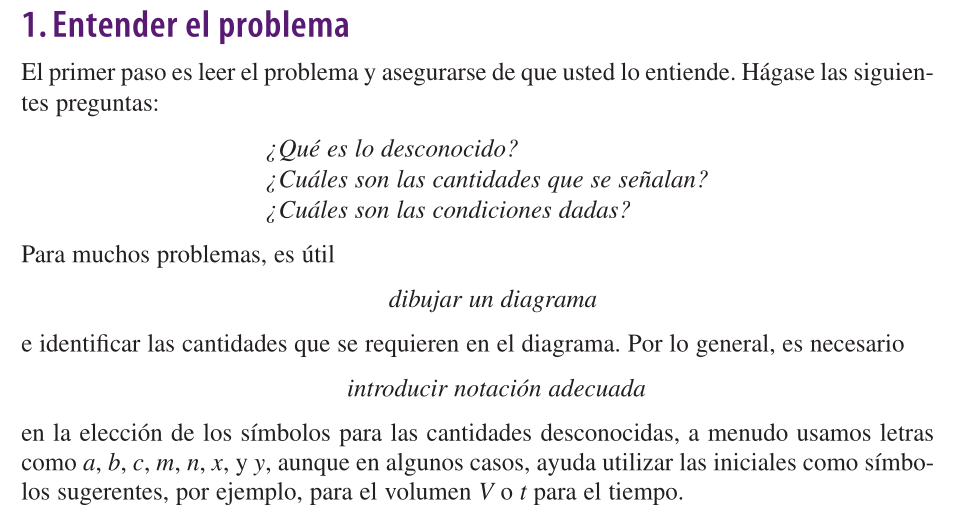
\includegraphics[width=0.7\textwidth,height=\textheight]{image.png}

\begin{center}\rule{0.5\linewidth}{0.5pt}\end{center}

\section{Ejemplo}\label{ejemplo}

\textbf{Rapidez promedio} Una conductora se embarca en un viaje. Durante
la primera mitad de la distancia, ella conduce al ritmo pausado de
\(30 km/h\), durante la segunda mitad conduce a \(60 km/h\). ¿Cuál es su
rapidez promedio en este viaje?

\begin{center}\rule{0.5\linewidth}{0.5pt}\end{center}

\textbf{\emph{¿Cual es la solución?}}

\begin{center}\rule{0.5\linewidth}{0.5pt}\end{center}

\subsection{Paso 1: Definir las
variables}\label{paso-1-definir-las-variables}

Denotemos la distancia total del viaje como \$ D \$. Entonces, cada
mitad de la distancia es \$ \frac{D}{2} \$.

\subsection{Paso 2: Calcular el tiempo para cada mitad del
viaje}\label{paso-2-calcular-el-tiempo-para-cada-mitad-del-viaje}

Para la primera mitad de la distancia (\$ \frac{D}{2} \$) a una
velocidad de \(30 km/h\):
\[t_1 = \frac{\frac{D}{2}}{30} = \frac{D}{60} \text{ horas}\]

Para la segunda mitad de la distancia (\$ \frac{D}{2} \$) a una
velocidad de 60 km/h:

\[t_2 = \frac{\frac{D}{2}}{60} = \frac{D}{120} \text{ horas}\]

\begin{center}\rule{0.5\linewidth}{0.5pt}\end{center}

\subsection{Paso 3: Calcular el tiempo total del
viaje}\label{paso-3-calcular-el-tiempo-total-del-viaje}

El tiempo total del viaje es la suma de los tiempos para cada mitad:
\[t_{\text{total}} = t_1 + t_2 = \frac{D}{60} + \frac{D}{120}\]

Para sumar estas fracciones, encontramos un denominador común:

\[t_{\text{total}} = \frac{2D}{120} + \frac{D}{120} = \frac{3D}{120} = \frac{D}{40} \text{ horas}\]

\begin{center}\rule{0.5\linewidth}{0.5pt}\end{center}

\subsection{Paso 4: Calcular la velocidad
promedio}\label{paso-4-calcular-la-velocidad-promedio}

La velocidad promedio \$ v\_\{\text{promedio}\}\$ se define como la
distancia total dividida por el tiempo total:

\[v_{\text{promedio}} = \frac{D}{t_{\text{total}}} = \frac{D}{\frac{D}{40}} = 40 \text{ km/h}\]

\begin{center}\rule{0.5\linewidth}{0.5pt}\end{center}

\textbf{Los numeros Reales}

\begin{itemize}
\tightlist
\item
  Números naturales
\item
  Números enteros
\item
  Números racionales
\item
  Números irracionales
\item
  Números reales
\end{itemize}

\begin{center}\rule{0.5\linewidth}{0.5pt}\end{center}

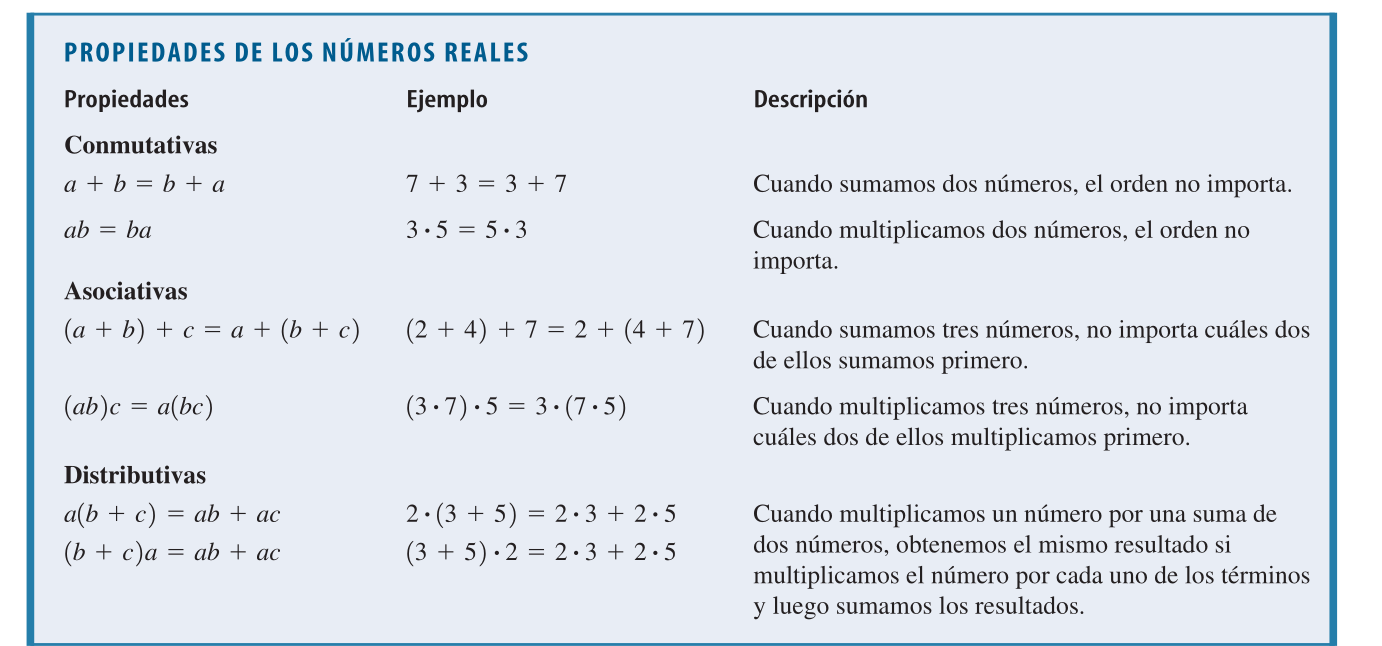
\includegraphics[width=0.7\textwidth,height=\textheight]{propiedades.png}

\begin{center}\rule{0.5\linewidth}{0.5pt}\end{center}

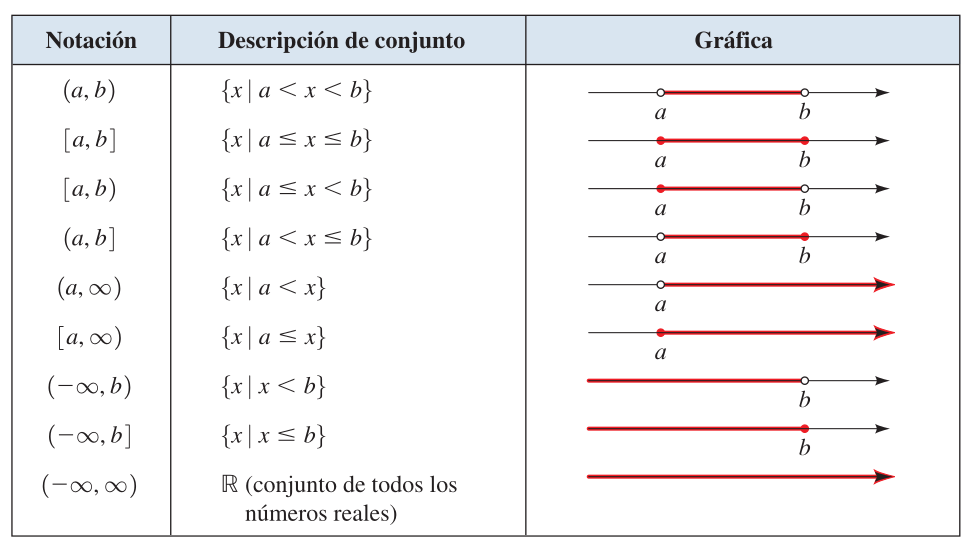
\includegraphics[width=0.7\textwidth,height=\textheight]{intervalos.png}

\begin{center}\rule{0.5\linewidth}{0.5pt}\end{center}

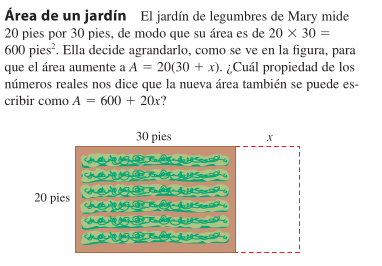
\includegraphics[width=0.7\textwidth,height=\textheight]{problema1.png}

\begin{center}\rule{0.5\linewidth}{0.5pt}\end{center}

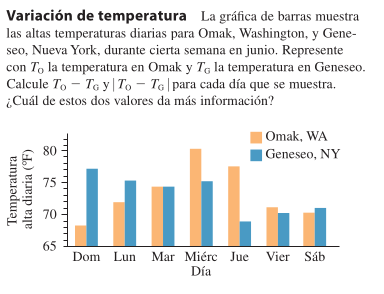
\includegraphics[width=0.7\textwidth,height=\textheight]{problema2.png}

\begin{center}\rule{0.5\linewidth}{0.5pt}\end{center}

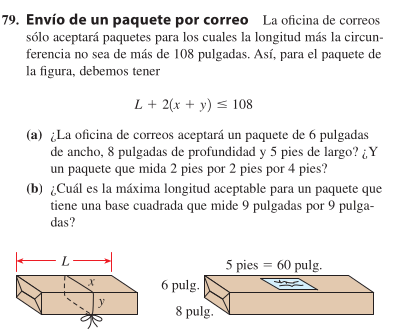
\includegraphics[width=0.7\textwidth,height=\textheight]{problema3.png}




\end{document}
